\documentclass[10pt,a4paper]{article}
\usepackage[utf8]{inputenc}
\usepackage[german]{babel}
\usepackage[T1]{fontenc}
\usepackage{amsmath}
\usepackage{amsfonts}
\usepackage{amssymb}
\usepackage{graphicx}
\usepackage{listings}
\usepackage{color}
\usepackage{upquote}
\author{Julian Sobott (76511), David Sugar (76050), Lukas Mendel (76509)}
\title{Bericht Datenbank Praktikum}



\usepackage{geometry}
 \geometry{
 a4paper,
 total={170mm,257mm},
 left=20mm,
 top=20mm,
 }


\lstset{
	language=sql,
	tabsize=4,
	keywordstyle=\color{blue},
	breaklines=true,
        moredelim=[is][\underbar]{@}{@}
}	
\begin{document}
\maketitle
\tableofcontents

\newpage
\section{Aufgabe 1: Entwurf und Implementierung des Datenmodells}
\subsection{a) ERM}

\begin{figure}[ht!]
	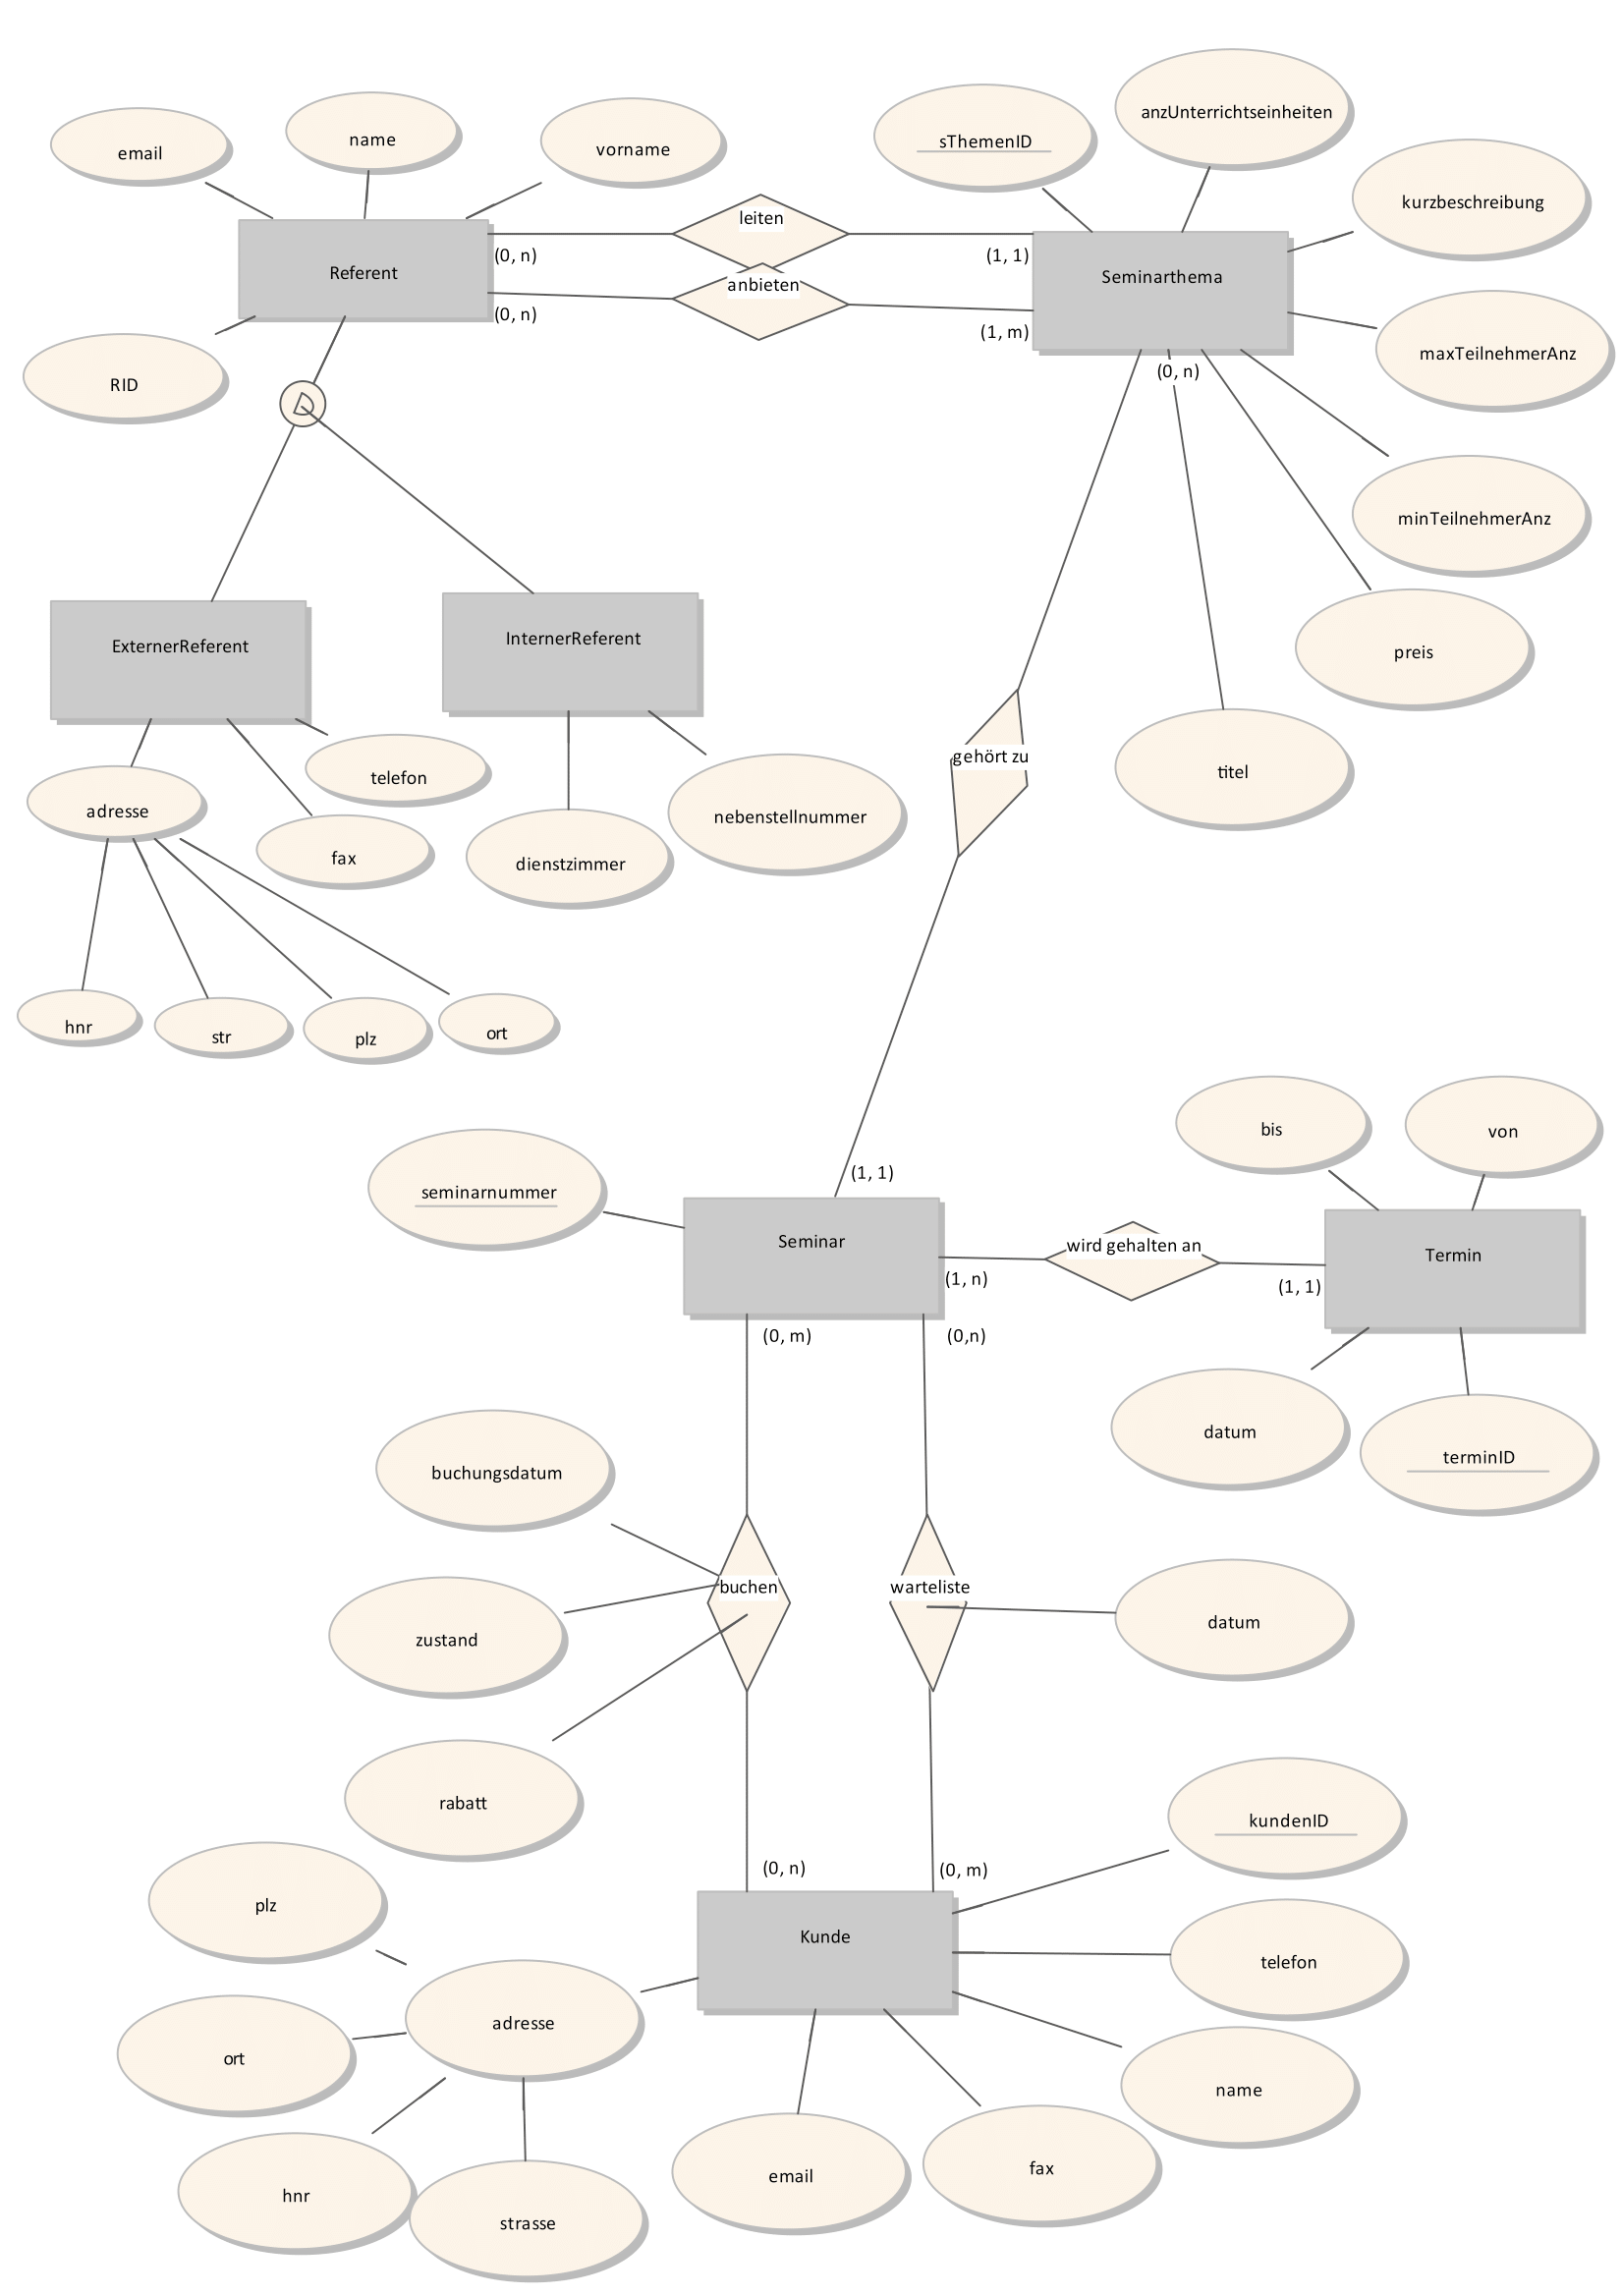
\includegraphics[scale=0.2]{Bilder/ER-Modell.PNG}
	\caption{ER-Modell Seminarverwaltung}
	\label{er:1}
\end{figure}

\subsubsection{Beschreibung des Modells}

\textbf{is\_a Beziehung zwischen Referenten:} Aufgrund der Tatsache, dass alle Referenten sowohl gemeinsame als auch verschiedene Attribute haben, 
haben wir uns für eine disjunkte Spezialisierung entschieden. Das heißt die gemeinsamen Attribute sind in der 
generellen Entity Referent und nur die speziellen Attribute sind in den Spezialisierungen Externer Referent und
Interner Referent.
\\
\textbf{Beziehung zwischen Referent und Seminarthema:} Da zwischen einem Seminar leiten und einem Seminar anbiten 
unterschieden wird, haben wir uns für zwei Relationen zwischen Referent und Seminarthema entschieden.
\\
\textbf{Beziehung zwischen Seminar und Kunde:} Selbiges gilt in dieser Beziehung. Ein Kunde kann sowohl ein Seminar buchen 
als auch in einer Warteliste landen.
\\
\textbf{Beziehung zwischen Seminarthema und Seminar:} Es kann mehrere Veranstaltungen (Seminare) zu einem Seminarthema geben. Wobei ein Seminar immer nur über ein Seminarthema geht.
\\
\textbf{Beziehung zwischen Seminar und Termin:} Da ein Seminar an mehreren Terminen stattfinden kann, wurde der Termin in eine extra Entity ausgelagert.


\subsubsection{Unterschiede zum UML Modell}

\begin{itemize}

\item Im UML Diagramm wurde das Listenmodell zwischen Seminar und Termin verwendet. Dies ist im ERM aber nicht möglich und ist stattdessen eine Relation.
\item Die Beziehung zwischen Seminarthema und Seminar ist die gleiche, nur statt Exemplartyp wurde eine Relation verwendet.
\item Im UML wird mithilfe von Vererbung eine Klasse um die benötigten Attribute erweitertt, um eine Spezialisierung zu erreichen.
 Im ERM hingegen wird über eine is\_a Beziehung eine Spezialisierung realisiert.
\item Im UML wurde eine Koordinatorklasse für die Buchungen verwendet. Im ERM hingegen wird hier eine Relation mit Attributen verwendet.
\item Anstatt der \textit{ordered} Constraint wird im ERM eine Relation genommen, die das Datum speichert. Durch das Datum kann eine Ordnung hergestellt werden.

\end{itemize}


\newpage

\subsubsection{Entities}
\begin{lstlisting}[]
seminar = ({@seminarnummer@:Integer})

termin = ({@terminid@:Integer, datum:Date, von:DateTime, bis:DateTime})

kunde = ({@kundenid@:Integer, telefon:Varchar, name:Varchar, fax:Varchar, email:Varchar, adresse:(plz:Varchar, ort:Varchar, hnr:Varchar, str:Varchar)})  

referent = ({@rid@:Integer, email:Varchar, name:Varchar, vorname:Varchar})

seminarthema = ({@sthemaid@:Integer, anzunterichtseinheiten:Integer, kurzbeschreibung:Varchar, maxteilnehmeranz:Integer, minteilnehmeranz:Integer, preis:Float, titel:Varchar})

externerReferent = ({@rid@:Integer, adresse:(strasse:Varchar, hnr:Varchar, plz:Varchar, ort:Varchar)

internerReferent = ({@rid@:Integer, dienstzimmer:Varchar, nebenstellnummer:Integer})
\end{lstlisting}

\subsubsection{Relations}
\begin{lstlisting}[]
leiten = (referent x seminarthema)

anbieten = (referent x seminarthema)

gehört_zu = (seminarthema x seminar)

buchen = (seminar x kunde, buchungsdatum:Date, zustand:Varchar, rabatt:Float)

warteliste = (kunde x seminar, datum:Date)

wird_gehalten_an = (seminar x termin)
\end{lstlisting}

\subsection{b) Relationales Modell}
\subsubsection{Relations}

\begin{lstlisting}[]
referent = (@rid@:Integer, email:Varchar, name:Varchar, vorname:Varchar)

externerReferent = (@rid@:Integer, strasse:Varchar, hnr:Varchar, plz:Varchar, ort:Varchar)

internerReferent = (@rid@:Integer, dienstzimmer:Varchar, nebenstellnummer:Integer)

seminarthame = (@sthemaid@:Integer, anzunterichtseinheiten:Integer, kurzbeschreibung:Varchar, maxteilnehmeranz:Integer, minteilnehmeranz:Integer, preis:Float, titel:Varchar, leiter:Integer)

anbieten = (@referentid@:Integer, seminarthemaid:Integer)

seminar = (@seminarnummer@:Integer, seminarthemaid:Integer)

termin = (@terminid@:Integer, von:Datetime, bis:Datetime, datum:Date, seminarid:Integer)

kunde = (@kundenid@:Integer, telefon:Varchar, name:Varchar, fax:Varchar, email:Varchar, plz:Varchar, ort:Varchar, hnr:Varchar, str:Varchar)

buchen = (@kundenid@:Integer, seminarnr:Integer, buchungsdatum:Date, zustand:Varchar, rabatt:Float)

warteliste = (@kundenid@:Integer, seminarnr:Integer, datum:Date)
\end{lstlisting}

\subsubsection{Referenzen}
$seminarthema\vert_{LEITER} \subseteq refernet\vert_{RID}$

$anbieten\vert_{REFERENTID} \subseteq refernet\vert_{RID}$

$anbieten\vert_{SEMINARTHEMAID} \subseteq seminarthema\vert_{STHEMAID}$

$seminar\vert_{SEMINARTHEMAID} \subseteq seminarthema\vert_{STHEMAID}$

$termin\vert_{SEMINARID} \subseteq seminar\vert_{SEMINARNUMMER}$

$buchen\vert_{KUNDENID} \subseteq kunde\vert_{KUNDENID}$

$buchen\vert_{SEMINARNR} \subseteq seminar\vert_{SEMINARNR}$

$warteliste\vert_{KUNDENID} \subseteq kunde\vert_{KUNDENID}$

$warteliste\vert_{SEMINARNR} \subseteq seminar\vert_{SEMINARNR}$

\subsection{c) SQL-Staments: create tables}

\lstinputlisting{../create_table_statements.sql}

\section{Aufgabe 2: SQL-Statements für das Einfügen von Datensätzen}
\lstinputlisting{../insert_table_statements.sql}

\section{Aufgabe 3: SQL-Statements für Datenabfrage}
\lstinputlisting{../SQL_Abfragen.sql}


% TODO: Aufgabe 3, check all sql_statements

\end{document}



